\section{Design}
The overarching target of \TheName is to capture all syscalls issued by target application with low overhead. Specifically, it has the following characteristics:

\begin{itemize}
    \item \textbf{online:} Our scenario is that our entire record system can  work simultaneously on the user side and eventually become a part of the log report. Therefore it must introduce only a extremely low overhead to guarantee that the user can run the desired program without perception.
    \item \textbf{complete:} We also need to ensure the integrity of record results, i.e. that every syscall is correctly captured with all the data needed for reproduction. Not only do we need to verify the correctness of our records on each syscall, but we also have to guarantee that the data in the buffer is fetched in a timely manner without any overflow.
    \item \textbf{off-the-shore:} An practical system should never make assumptions about the hardware. \TheName is desgined completely based on the off-the-shelf hardware.
    \item \textbf{without modification to application:} We do not make any changes to the source code or binary of the target application. The entire code of our system runs in kernel space, except for the transfer of logged results that need to be transferred to user space. This means that \TheName cares nothing about how the target application in user space is executed, but only about the event that this target application jumps to the kernel state.
    \item \textbf{without modification to kernel:} Modifying Kernel source may make all procedures much more easy. However, this approach will inevitably reduce the compatibility of \TheName, especially for devices whose kernels have been modified by manufacturers. Futhermore, to modify kernel, we would also need to synchronize upstream changes. Consequently, \TheName is baesd on kernel moudle and works as a loadbale driver.
\end{itemize}


\TheName realizes syscall capturing in three steps. (1) \TheName inspect and record each syscall. (2) Next, \TheName filter these records by some arrtibutions of its caller process. (3) Finally, \TheName transfer these filtered records.

\begin{figure}
    \centering
    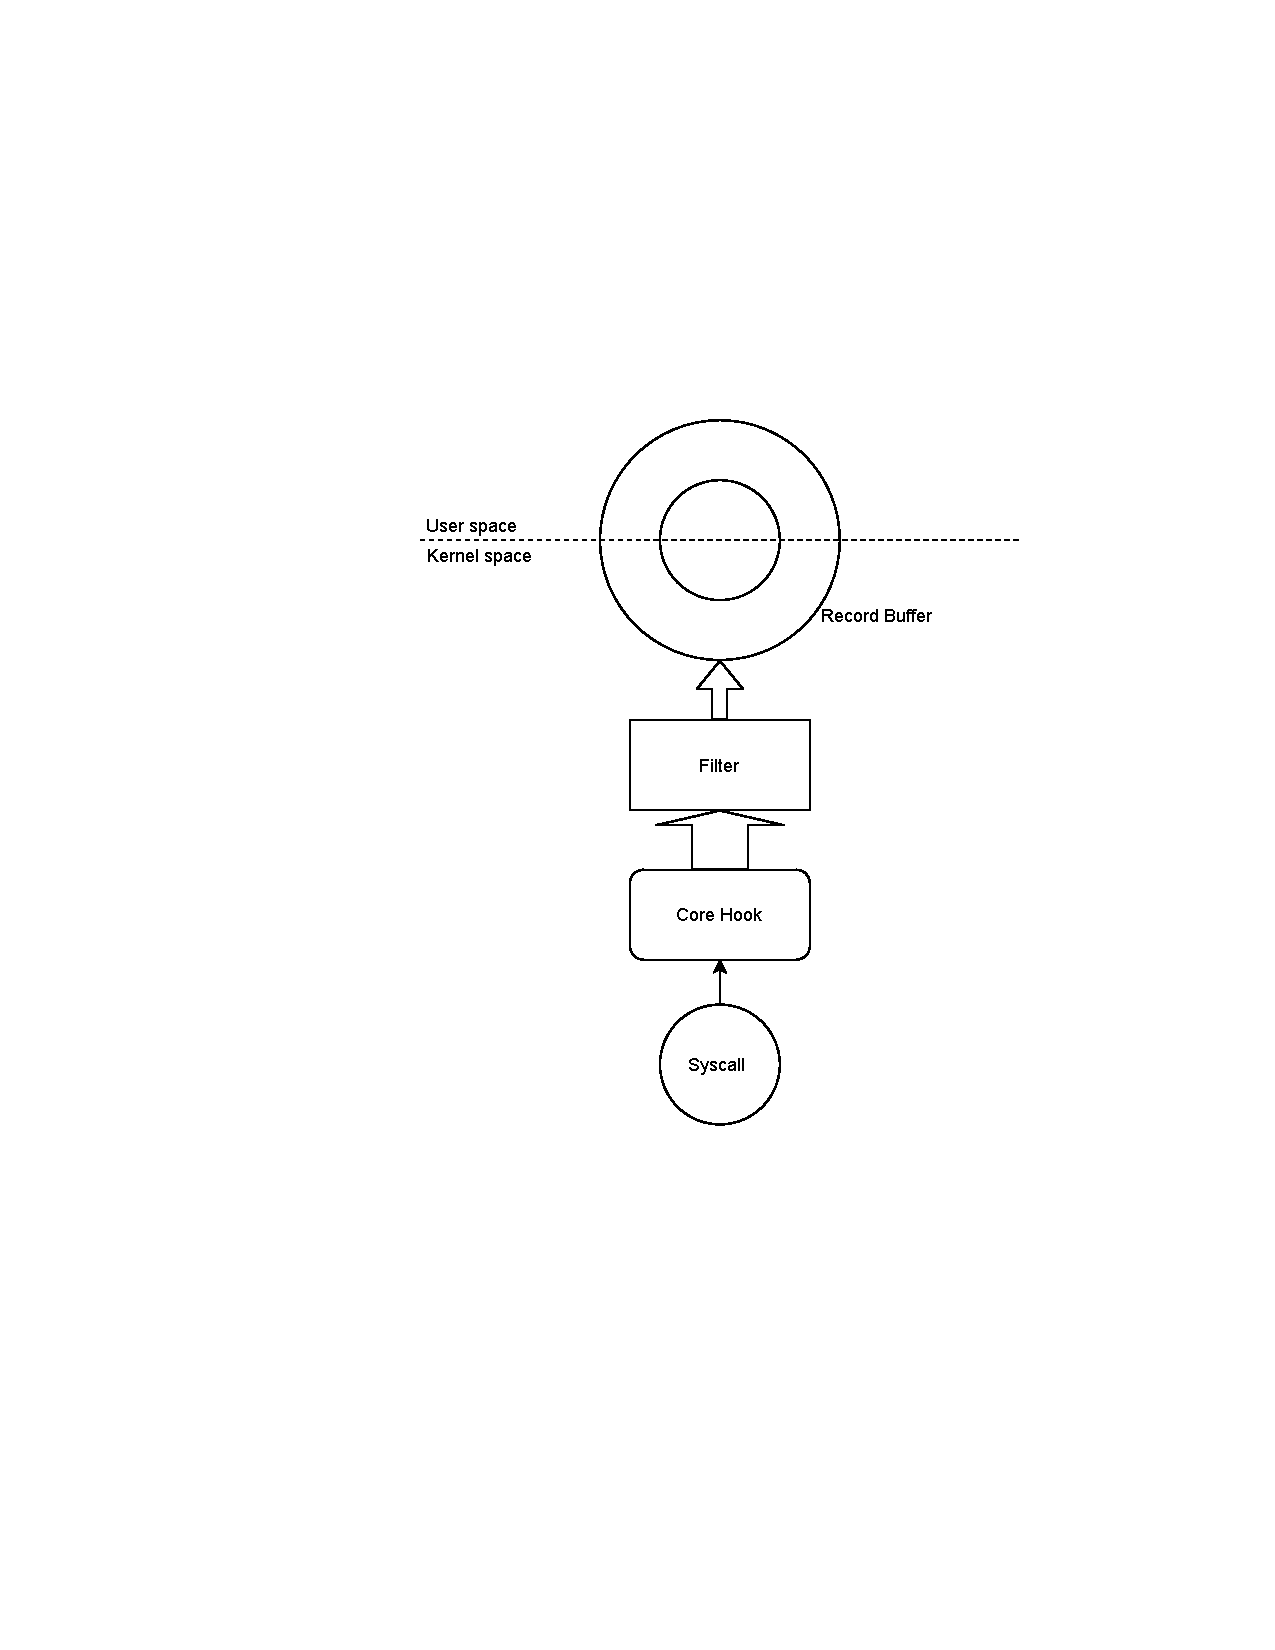
\includegraphics[width=0.8\textwidth]{figures/arch.pdf}
    \caption{The Overview of \TheName}
    \label{fig:arch}
\end{figure}



% In this section, I describe the desgin of \TheName by focusing on how it solves the above challenges

\subsection{Desgin Overview}

In this section, we present the desgin of \TheName by focusing on how it addresses the above two key challenges. \TheName contians three parts: \textit{core hook}, \textit{filter}, and \textit{record buffer}. 

As Figure \ref{fig:arch} shows, in the kernel space, \textit{core hook} collect information for each system call, and then transfer to \textit{filter} part. Subsequently, at the \textit{filter} part, it will find process information from the kernel, and filter syscall records with specific features (e.g., process id or name) and finally pass to \textit{record buffer}. The record buffer manage the buffer in kernel space and file write to user space.


\subsection{Case Study}

\begin{figure}
    \begin{minipage}[t]{0.46\textwidth}
      \begin{lstlisting}
  // Thread 1::
  char big_buf[64];
  while(1)
    read(fd, big_buf, 64);
      \end{lstlisting}    
    \end{minipage}
    \begin{minipage}[t]{0.46\textwidth}
      \lstset{firstnumber=last}
      \begin{lstlisting}
  // Thread 2::
  int total = 0;
  int len = 0;
  char buf[15];
  for (short i=0; i < 2; ++i)
    len = strlen(big_buf);
    if (len < 15)
      strcpy(buf, big_buf);
      total += len;
  assert(total<30)
    \end{lstlisting}    
    \end{minipage}
  
  
    \caption{Buffer Overflow Caused by Data Race}
    \label{fig:data-race}
\end{figure}

Figure~\ref{fig:data-race} demonstrates a typical concurrency
bug related to the non-deterministic event
(\syscall{} \texttt{read}). Assume that the loop (Line 10 to Line 13) in Thread 2
is executed twice. In the first iteration, the \texttt{read} of 
\texttt{big\_buf} (Line 4) in Thread 1 is performed after the length 
check (Line 10 and Line 11) in Thread 2. The following \texttt{strcpy} (Line 12) in 
Thread 2 may lead to a buffer overflow and overwrite variables \texttt{len} and 
\texttt{total}. In the second iteration, no data race is involved, but the 
unpredictable \texttt{total} overwritten in the first iteration might be larger
than 30 after the summation (Line 13) in Thread 2. This finally fails the
\texttt{assert} (Line 14) in Thread 2 and crashes the program.
In this example, the memory and registers indicating the root cause of
the bug are overridden by subsequent control flow. 
Hence, it is necessary to record the content of syscall \texttt{read} to figure out the bug.


\begin{figure}
    \centering
    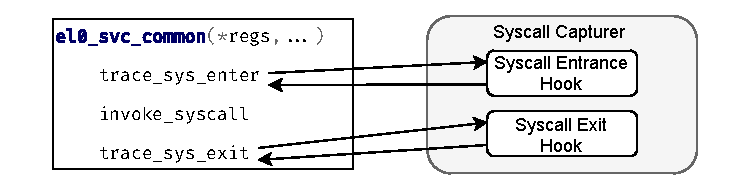
\includegraphics[width=0.95\textwidth]{figures/syscall_capturer.pdf}
    \caption{The Two hooks of \textit{core hook}}
    \label{fig:core-hook-desgin}
\end{figure}

\begin{table}
    % table caption should be in the top.
    \caption{
        Part of Registers Used in Syscalls \cite{syscall}.}
    \centering
    \begin{tabular}{lllllll}
        \toprule
        arch                      &  syscall number &
        return value &
        return value 2 & arg0                      & arg1 &
        arg2                                                               \\
        \midrule
        arm64                     & w8                        & x0   & x1
                                  & x0                        & x1   & x2  \\
        x86-64                    & rax                       & rax  &
        rdx                       & rdi                       & rsi  & rdx
        \\
        riscv                     & a7                        & a0   & a1
                                  & a0                        & a1   & a2  \\
        \bottomrule
    \end{tabular}
    \label{table:arch_registers}
\end{table}


\subsection{Core Hook}

\textit{Core hook} utilizes \textit{Linux Kernel Tracepoints} \cite{mathieu2021using}, which
provides lightweight hook points in critical positions over the kernel
(includes the enter and exit of \syscall{}), to achieve the capture.  Figure \ref{fig:core-hook-desgin} illustrates the procedure of \syscall{}s
(defined at function \texttt{el0\_svc\_\\common} for Arm64) and the recording for \syscall{}s. 


When entering a \syscall{}, the kernel goes into \textit{syscall entrance
hook} which stores values of involved registers. As Table
\ref{table:arch_registers} shows, the register \texttt{x0} and \texttt{x1} are used as both
parameters and return values of \syscall{}s on Arm64. Thus, these registers are
overwritten by return values during \syscall{} procedure. Consequently, we may not
obtain the \syscall{} parameters at the \textit{syscall exit hook} directly.
However, these parameters are critical in some cases. For example, as Figure
\ref{fig:data-race} demonstrates, the content of \texttt{big\_buf}, addressed by
the first parameter of \texttt{read}, is necessary for failure analysis.
Therefore, we need to record the corresponding parameter at the \textit{syscall
entrance hook}, and further record the content addressed by \texttt{big\_buf} at 
the \textit{syscall exit hook}.

Before exiting a \syscall{}, the kernel falls into \textit{syscall exit
hook}. This hook records different information for
various types of \syscall{}s. Firstly, if the capturer notices that a
\syscall{} only changes specific registers (e.g., \texttt{getpid} only changes
return value), it could selectively save information to reduce the size of
record file. Secondly, we need to record additional information for
certain \syscall{}s;
for example, the \syscall{} \texttt{read(int fd, void *buf, size\_t count)}
tries to fill \texttt{count} bytes to the memory region addressed by
\texttt{buf}. In this case, we have to notice and record the write to this
memory region. 

For a better understanding of the impact of \syscall{}s, we classify
them into four types according to their effect on memory and registers.

\begin{itemize}
\item
\noindent\textbf{R}\textit{eading} \textbf{S}\textit{tatus}: 
The \textit{RS-Type} \syscall{}s
aim to read information related to system status. The results of
these \syscall{}s may be transferred by the return value (e.g., \texttt{getpid}), 
a pointer (e.g., \texttt{getitimer}), or shared memory (e.g.,
\texttt{getrandom}). For all \syscall{}s
in this category, we can directly record the memory or register they changed.

\item
\noindent\textbf{W}\textit{riting} \textbf{S}\textit{tatus}: 
The WS-Type \syscall{}s
changes the status of the system. As the WS-Type \syscall{}s do not
directly change the memory and registers of the program, we ignore
them unless they fail and return an error code. 
For example, the \syscall{} \texttt{epoll\_create} in \texttt{epoll} API
is ignored, but the influence of \syscall{} \texttt{epoll\_wait} is
recorded since we classify it as an \textit{RS-Type} \syscall{}.

%we do not handle \syscall{}
%\texttt{epoll\_create} in \texttt{epoll} API, while we record the influence
%of \syscall{} \texttt{epoll\_wait} as we classify it as \textit{Get from OS}.

\item
\noindent\textbf{R}\textit{eading} \textbf{C}\textit{ontent}: 
The \textit{RC-Type} \syscall{}s read content from an external input, and the
handling of \textit{RC-Type} \syscall{}s is similar to that of \textit{RS-Type} 
\syscall{}s. However, since the content is usually much larger than
the status read in the \textit{RS-Type} \syscall{}s, we choose to
truncate the content and record only the first 256 bytes due to
performance requirements. Recording the entire content may become
impractical in extreme cases (e.g., data center with tremendous
uploads) as it results in a huge size of record file. 
Besides, we find that the truncated content is sufficient for bug diagnosis in
most cases. A further evaluation is discussed in
\S ??.

\item
\noindent\textbf{W}\textit{riting} \textbf{C}\textit{ontent}:
The \textit{WC-Type} \syscall{}s write content to an external source. We 
consider that they would not affect the execution status of the target
program. For example, the \syscall{} \texttt{write} is ignored, and
the written content is recorded if the \textit{RC-Type} \syscall{}
\texttt{read} is used to read from the source again.
%The content of \syscall{}s like \texttt{write} or
%\texttt{sendto} also no needs to record, unless it fails.
\end{itemize}



% Table \ref{table:arch_registers}, both first argument(\texttt{arg1}) and return value are saved in register \texttt{r0}, which means the parameter stored in \texttt{r0} will be replaced with return value before the syscall return to user. This results in the inability to directly record the chanegs only at the end of syscall handled in kernel. I solve this problem by adding an extra record for several syscalls.


% \subsubsection{Filter by Process}

% The capture needs filter by process due to the concurrency of the OS, i.e., interleaving with multiple processes. Thus, to distinguish the different syscall callers, \TheName has to add the caller's information for each syscall record. Accordingly, this challenge become \textit{how to get the process that issued the system call}. I address this challenge by inspecting a sepcial data structure in Linux kernel.

% \subsubsection{Record Buffer}

% System call records need to be stored in a buffer, while it is a very important issue when it comes to somehow get them from the buffer in real-time, completely, and with low overhead. However, the most strightforward solution, i.e., trying to keep fetching data from the buffer and save to file, causes a huge amount of overhead. Therefore, I choose to directly write to file 



\subsection{Filter}

The \Filter is responsible for checking the issuer of the system call, then comparing it with the conditions passed in at load time, and finally passing the records that satisfy the conditions to the buffer.
\Filter leverages \texttt{current} to collect relevant information about the issuer. The \texttt{current} points to the process descriptor \texttt{task\_struct} which contains all the information about the executing process. During a procedure of system call, \texttt{current} pointer indicates the issuer \cite{corbet_linux_2005}. 



\subsection{Record Buffer}

The \textit{record buffer} is intended to act as a transit between kernel space and user space. One of the simplest designs is to maintain a daemon in user space constantly querying and retrieving the data stored in the buffer, and then dumping the data to a file. However, we note that this introduces a huge amount of overhead, mainly due to frequent file I/O. Placing a larger buffer in user space would also solve this problem, but \TheName does not want to introduce a large impact on the system.

Therefore, \TheName directly writes to file from the kernel, i.e., when the buffer is full, \TheName dumps the buffer to files. In addition, it is noticeable that the kernel can not write files in all cases. For example, considering system calls that controls files such as \texttt{open}, \texttt{read} or \texttt{close}, \TheName should avoid writing files, or it will induce scheduling while atomic. Hence, \TheName maintains an additional secondary buffer. When the original buffer uses up, its content transfers to the secondary buffer, and then waits for a syscall irrelevant to file management to dumps to file.